\chapter{Experimentation, Results and\\ Discussion}\label{chap:Results}

To prove the concept of an educational, embedded, audio radar, the system as a whole needed to be tested in situations where the results can be useful, not only to the user but also to future projects. The two functionalities of the radar were tested not under lab conditions but real-world situations.

\section{Continuous Wave}
\subsection{Test 1}
\subsubsection{Setup}

The radar was set up next to a busy road (\href{https://www.google.com/maps/place/2A+Kei+Rd,+Milnerton,+Cape+Town,+7441/@-33.88786,18.4880057,18z/data=!3m1!4b1!4m13!1m7!3m6!1s0x1c3367685d1feaef:0x496954106fdbf460!2sR27!3b1!8m2!3d-33.860762!4d18.5008175!3m4!1s0x1dcc5c266817aa89:0xc42b15917dc67735!8m2!3d-33.88786!4d18.4891}{Marine Drive, Milnerton}) on a pedestrian caution sign facing the traffic at an angle of $20^\circ$. The tone was set to $7000\ Hz$ and the duration of $3\ s$. The radar was powered by a power bank and the web interface controlled using an iPad. Figure \ref{fig:setup1} shows the setup next to the road.

\begin{figure}[h!]
    \centering
    {\begin{minipage}{0.45\textwidth}
        \centering
        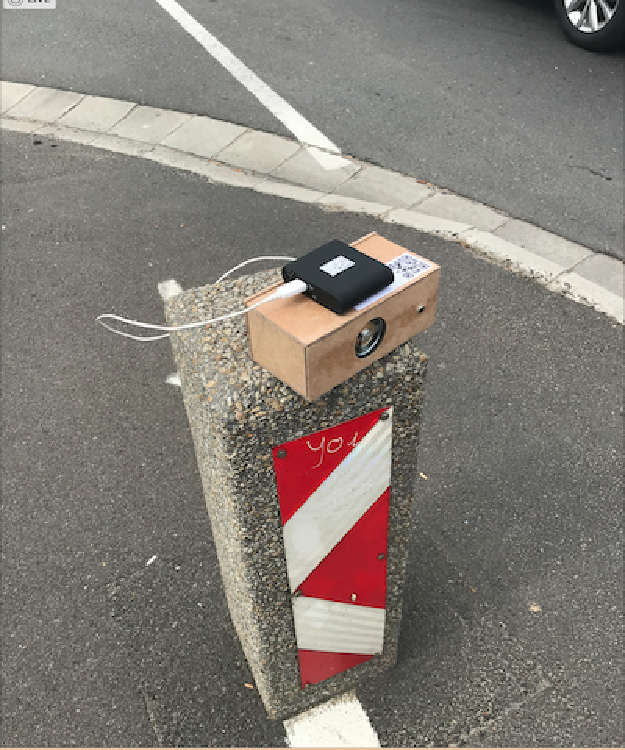
\includegraphics[width = 0.9\textwidth]{images/setup1.pdf}
    \end{minipage}\hfill
    \begin{minipage}{0.45\textwidth}
        \centering
        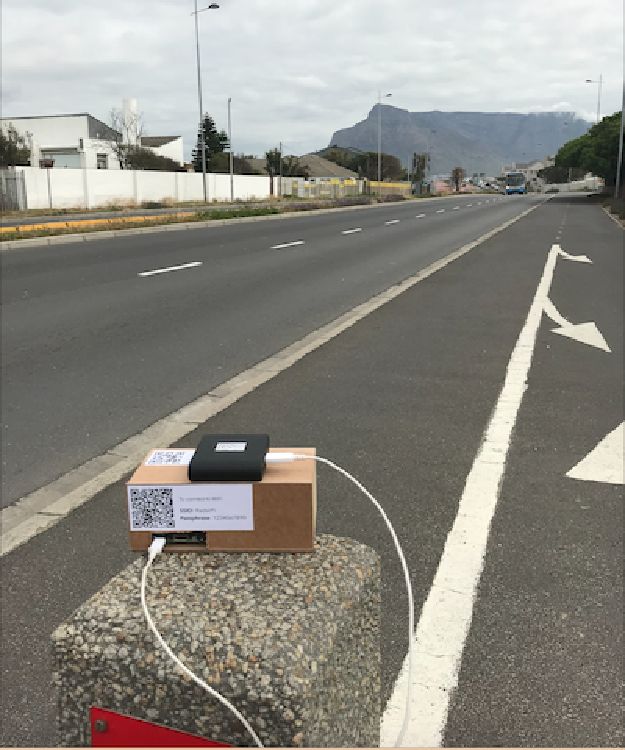
\includegraphics[width=0.9\textwidth]{images/setup2.pdf}
    \end{minipage}}\caption{Setup of CW Radar}\label{fig:setup1}
\end{figure}

\subsubsection{Result}
The results of the tests were not as successful as originally hoped for. The velocity of the vehicles is roughly $60\ km/h$, since the speed limit on this section is $60\ km/h$, which translates to $16.67\ m.s^{-1}$ and furthermore equates to a Doppler Frequency of approaching vehicles to be $8408.7\ Hz$ using Equation \ref{eq:dopplerEffect}. The Doppler Frequency, and hence the velocity, is at an angle and the radial velocity toward the radar can be calculated using trigonometry. The radial velocity is calculated using Equation \ref{eq:trig}. The results obtained for this setup can be seen in Figure \ref{fig:trig}. The resulting spectrograms for two vehicles following each other can be seen in Figures \ref{fig:resultsCW1} and \ref{fig:resultsCW2}.

\begin{figure}[h!]
    \centering
    \begin{minipage}{0.45\textwidth}
        \centering
        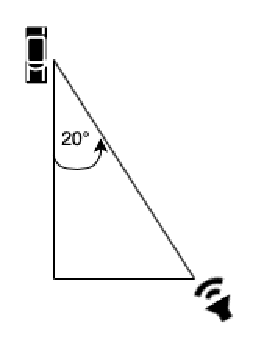
\includegraphics[width=0.75\textwidth]{images/trig.pdf}
        \caption{Trigonometry for Velocity Measurement}\label{fig:trig}
    \end{minipage}
    \begin{minipage}{0.45\textwidth}
        \begin{equation}
        v_{actual} = v_{measured}\ cos(20^{\circ})\label{eq:trig}
        \end{equation}
    \end{minipage}\hfill
\end{figure}

\begin{figure}[h!]
    \centering
    \begin{minipage}{0.45\textwidth}
        \centering
        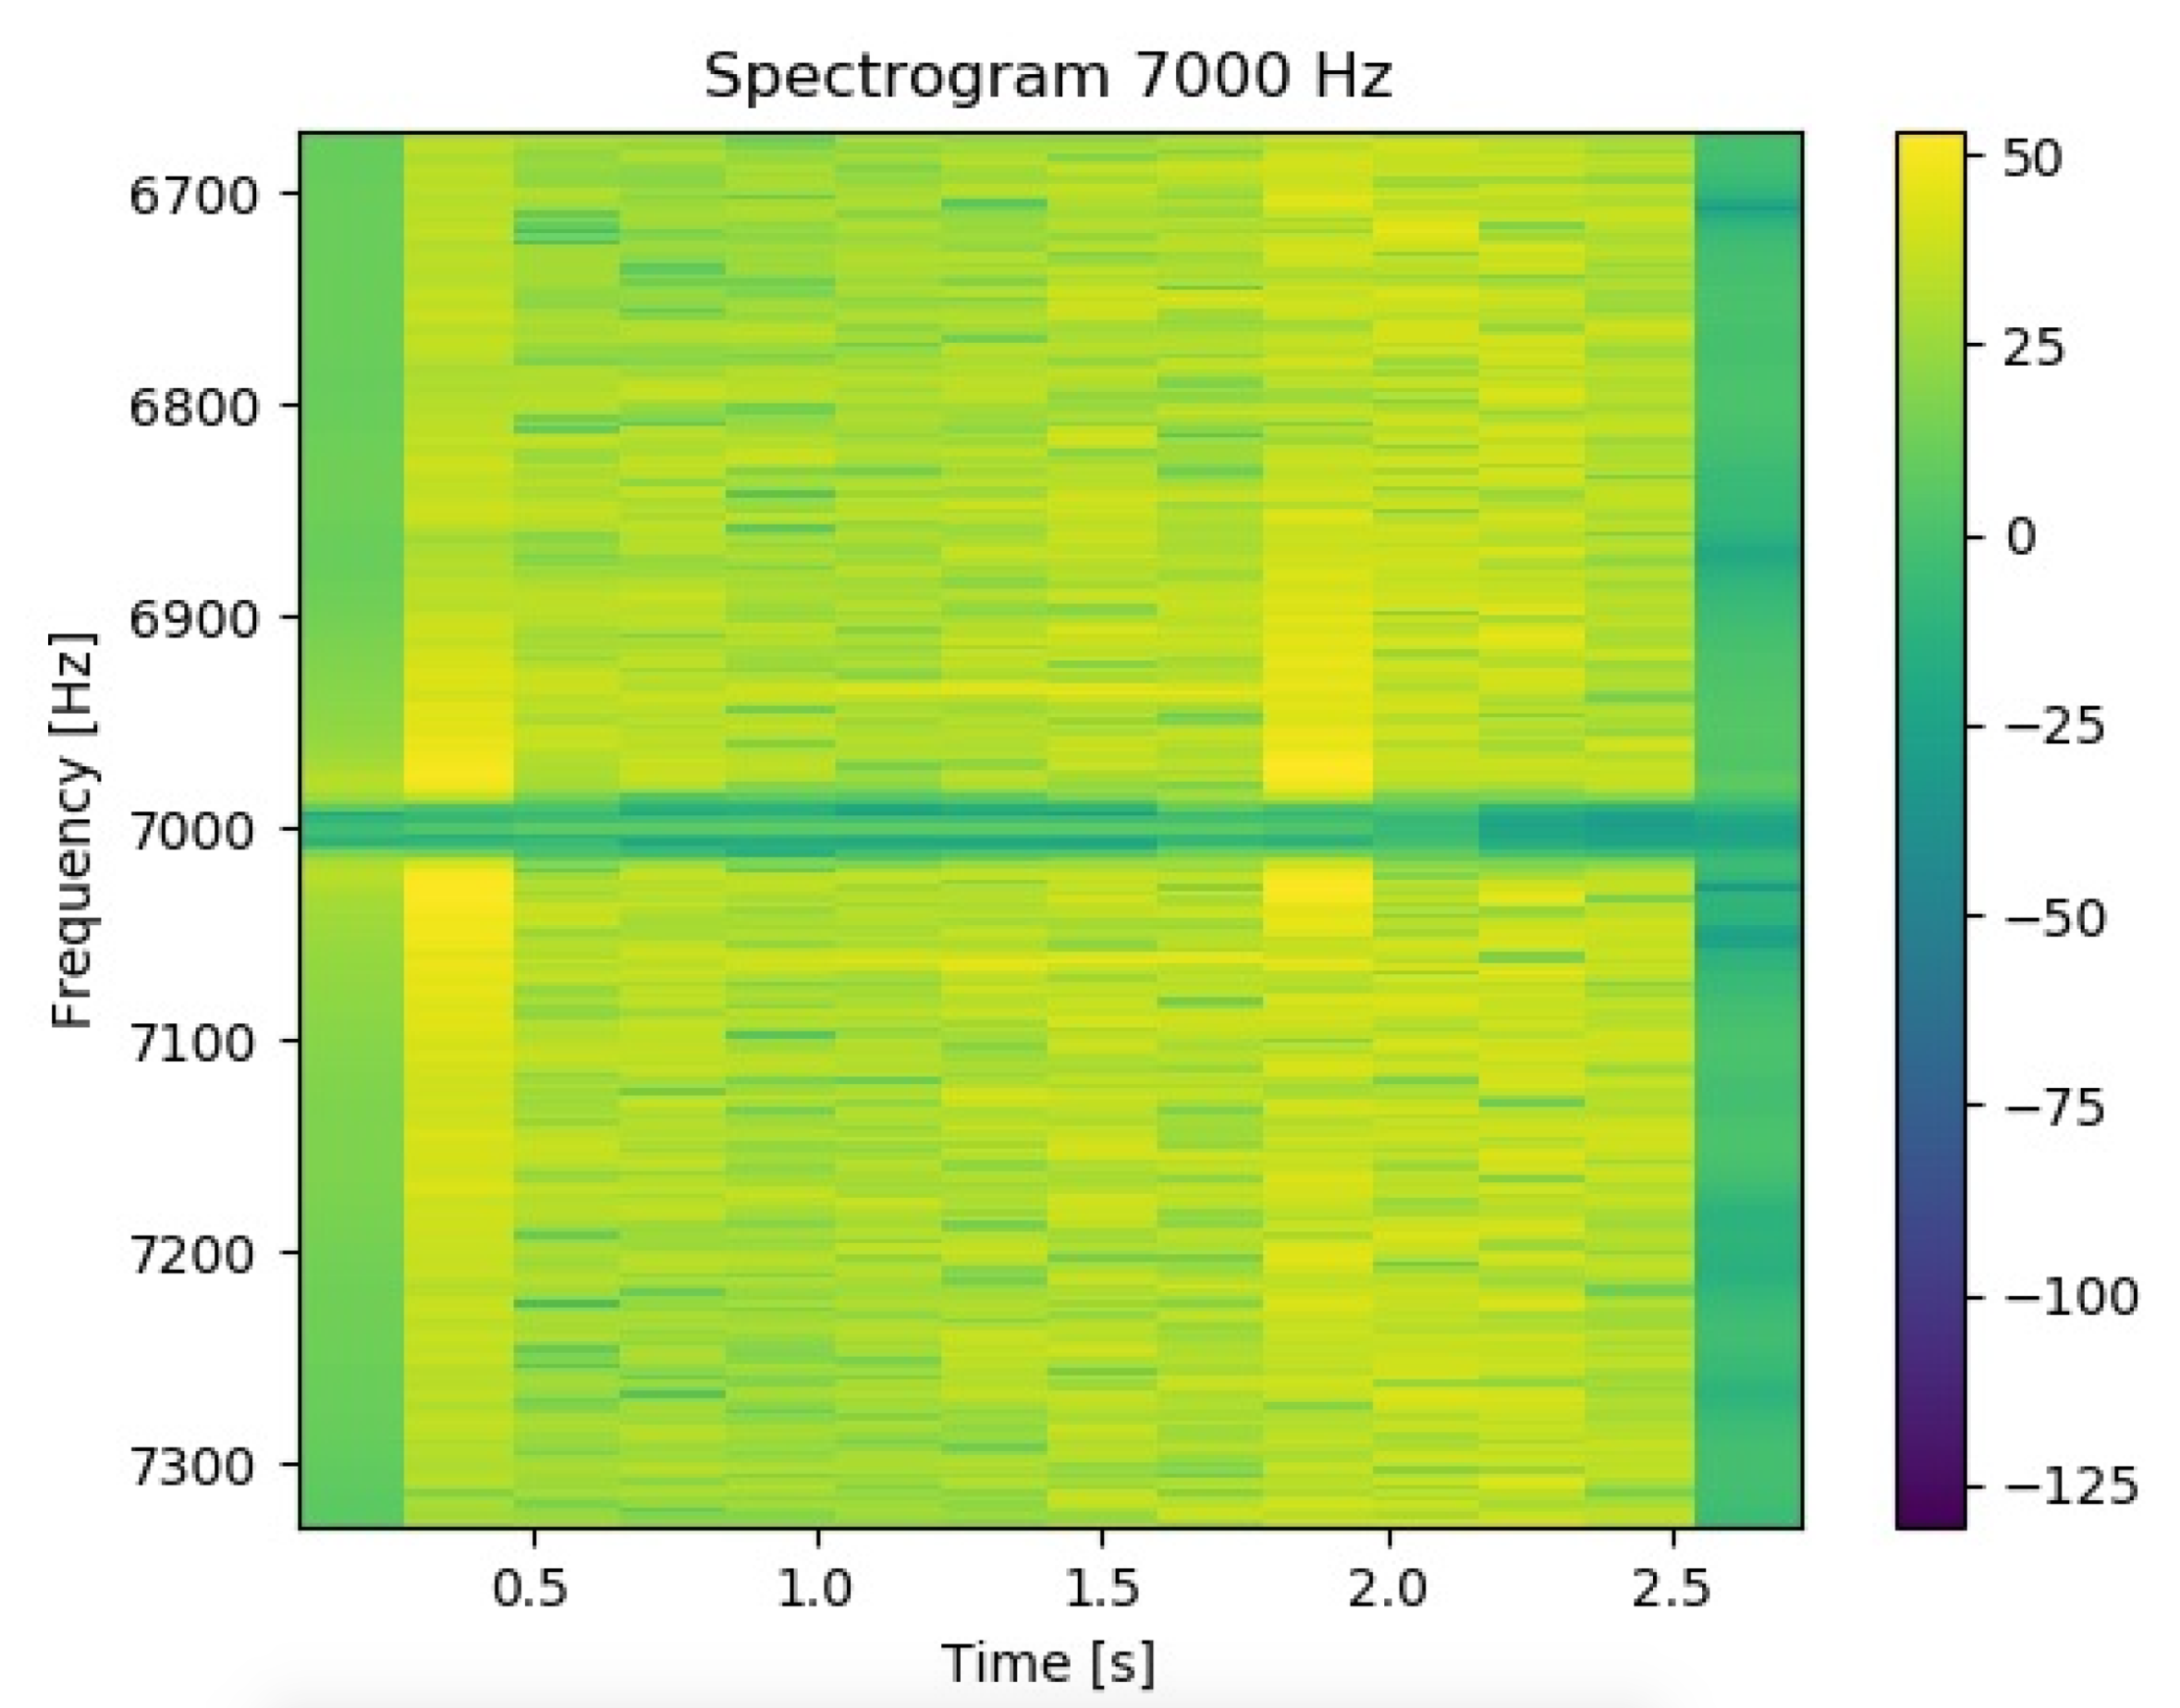
\includegraphics[width = 0.9\textwidth]{images/resultsCW1.pdf}
        \caption{Spectrogram of Cars driving CW Test 1}\label{fig:resultsCW1}
    \end{minipage}\hfill
    \begin{minipage}{0.45\textwidth}
        \centering
        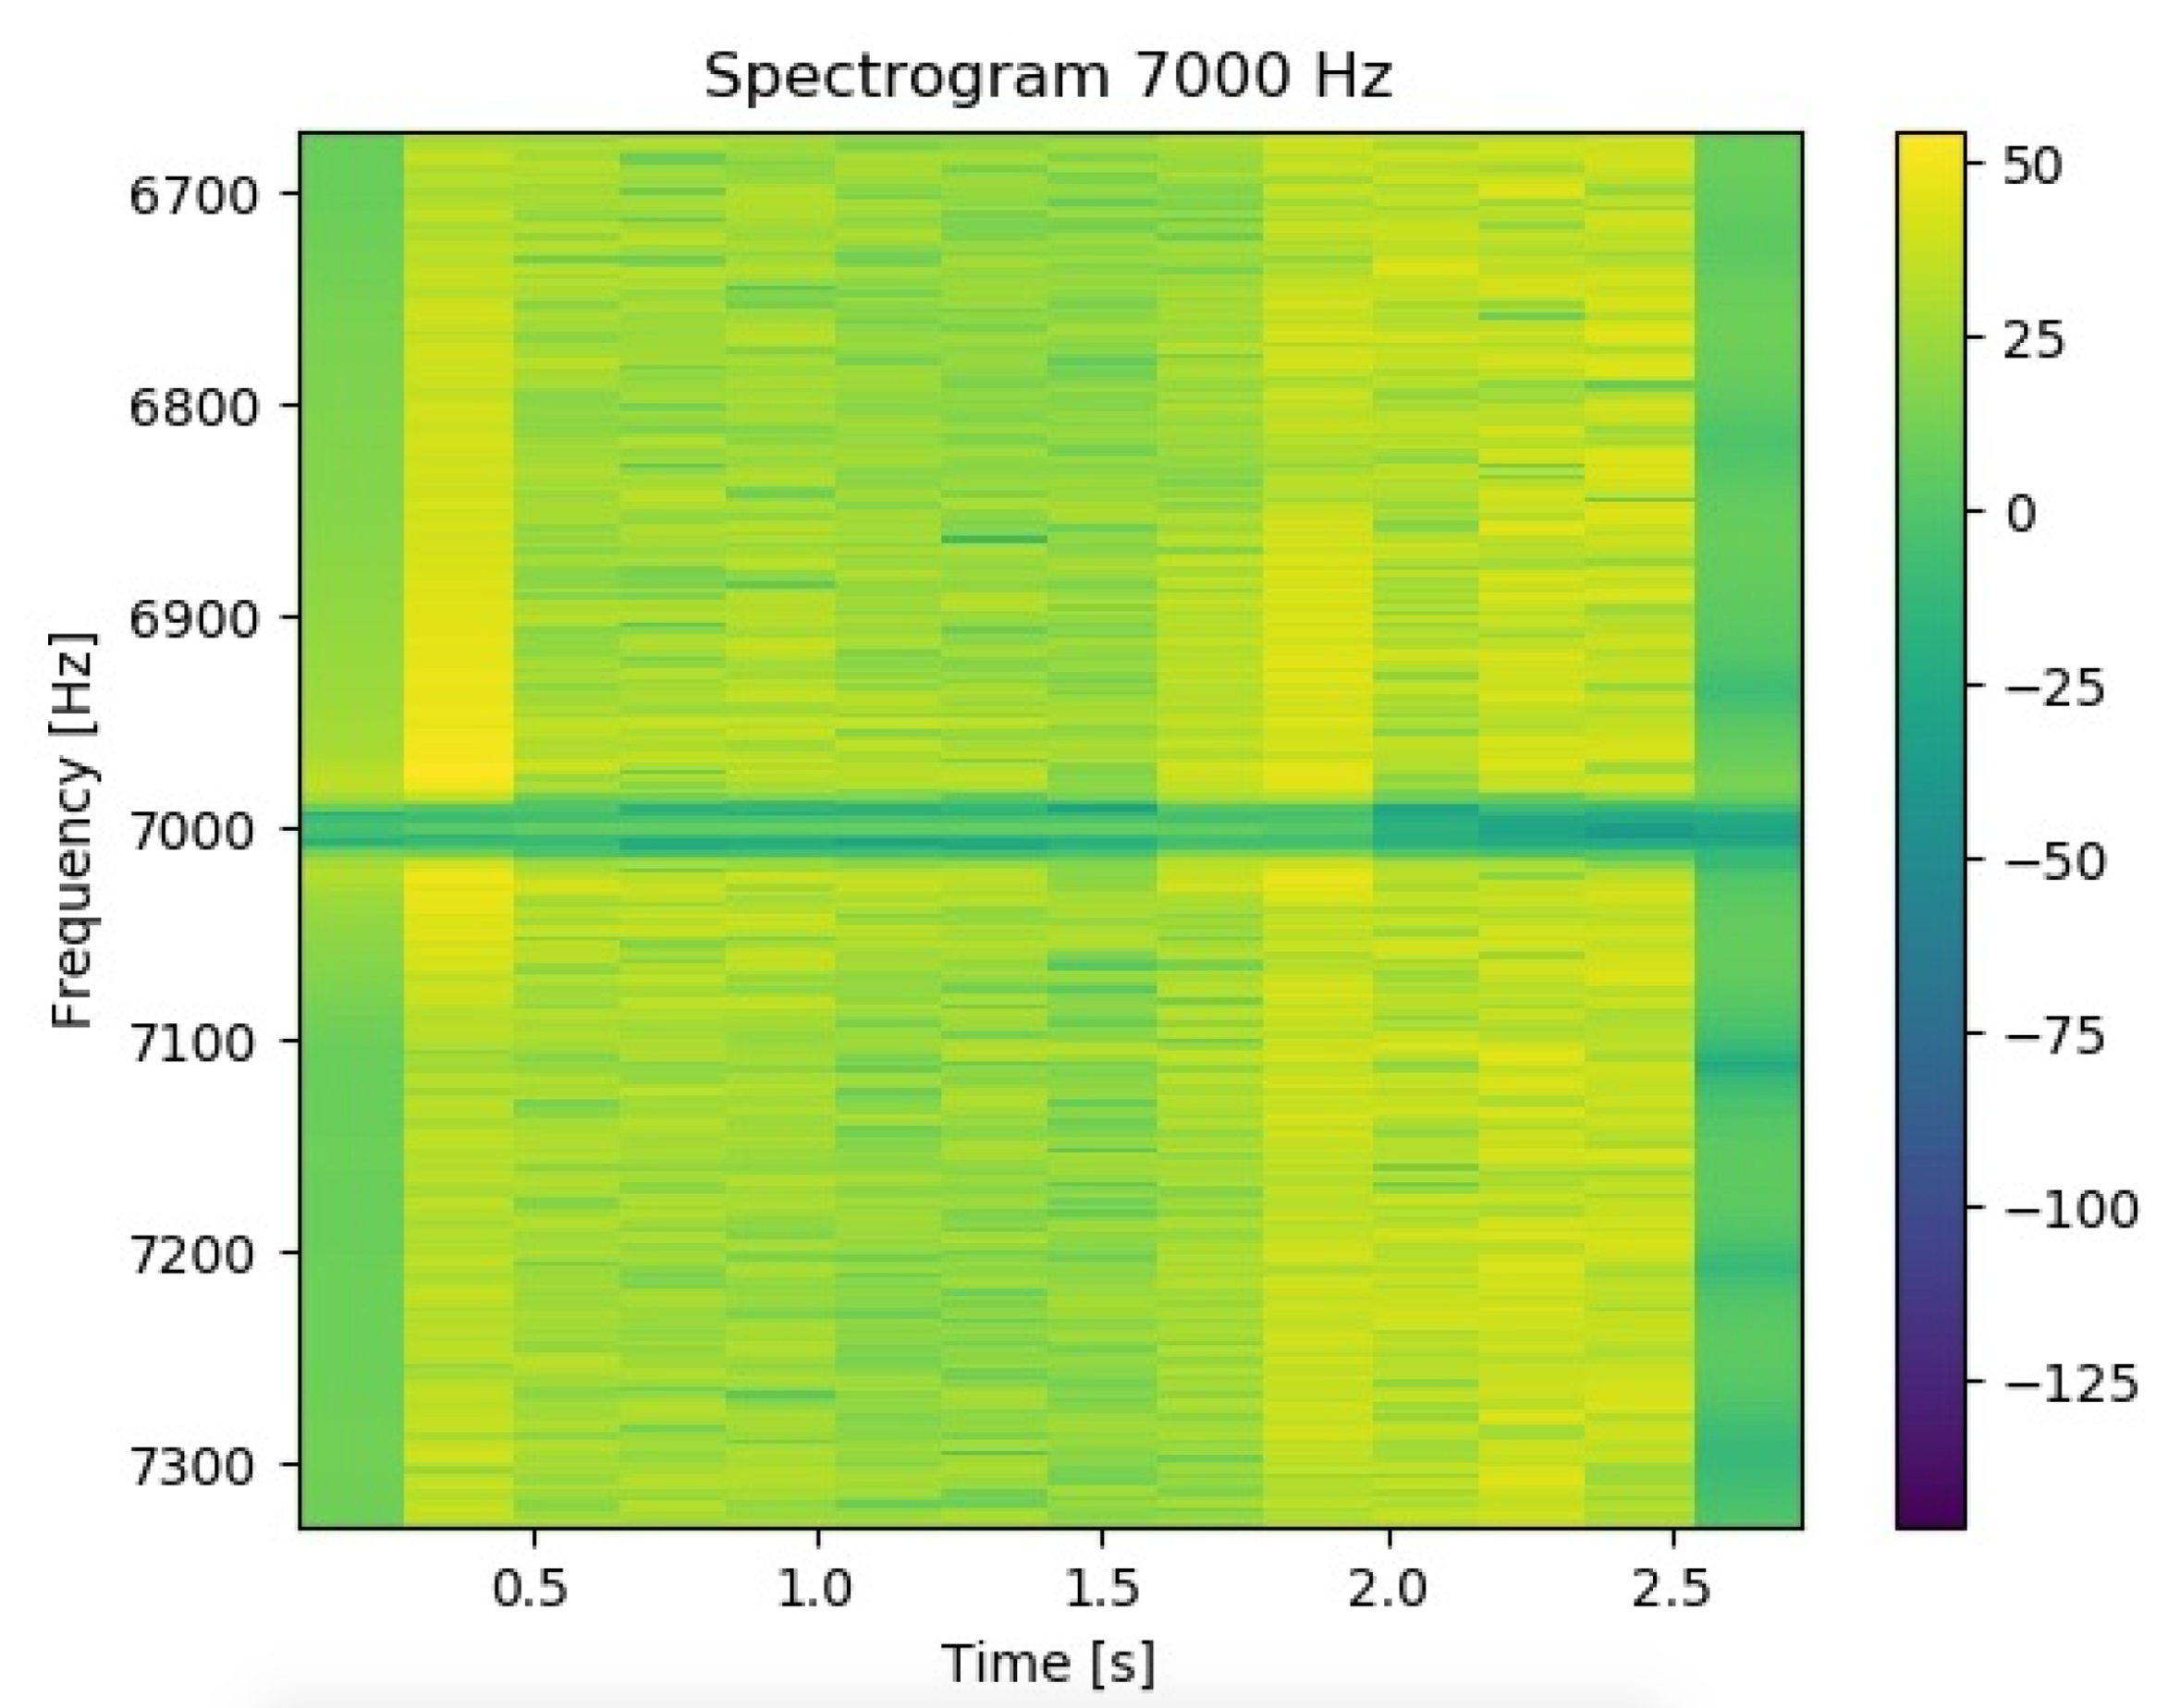
\includegraphics[width=0.9\textwidth]{images/resultsCW2.pdf}
        \caption{Spectrogram of Cars driving CW Test 2}\label{fig:resultsCW2}
    \end{minipage}
\end{figure}

\subsubsection{Discussion}
As shown above, the results are not as clear as initially intended. Figure \ref{fig:resultsCW1} shows a faint line around $7200\ Hz$ which translates to a rough estimate of the real velocity of $36\ km/h$. The line is decreasing in frequency and speaks to the fact that cars are speeding up as they accelerate from the traffic light down the road.

Figure \ref{fig:resultsCW2} however, shows only faint lines in the spectrogram with no significant features. This can be attributed to the loud ambient noises surrounding the radar including car engines, nearby construction and the automatic gain of the microphone highlighting even the quietest noise at a distance.


\subsection{Test 2}
\subsubsection{Setup}
The second test performed using the continuous wave radar was measuring the velocity of a golf club as it hits the ball off of a tee. The radar was placed $1\ m$ behind the tee and using a frequency of $7000\ Hz$ and $9000\ Hz$ and duration of $3\ s$ to capture both the backswing and forward swing of a single stroke. The setup of the test can be seen in Figure \ref{fig:golfball}.

\begin{figure}[h!]
    \centering
    \begin{minipage}{0.45\textwidth}
        \centering
        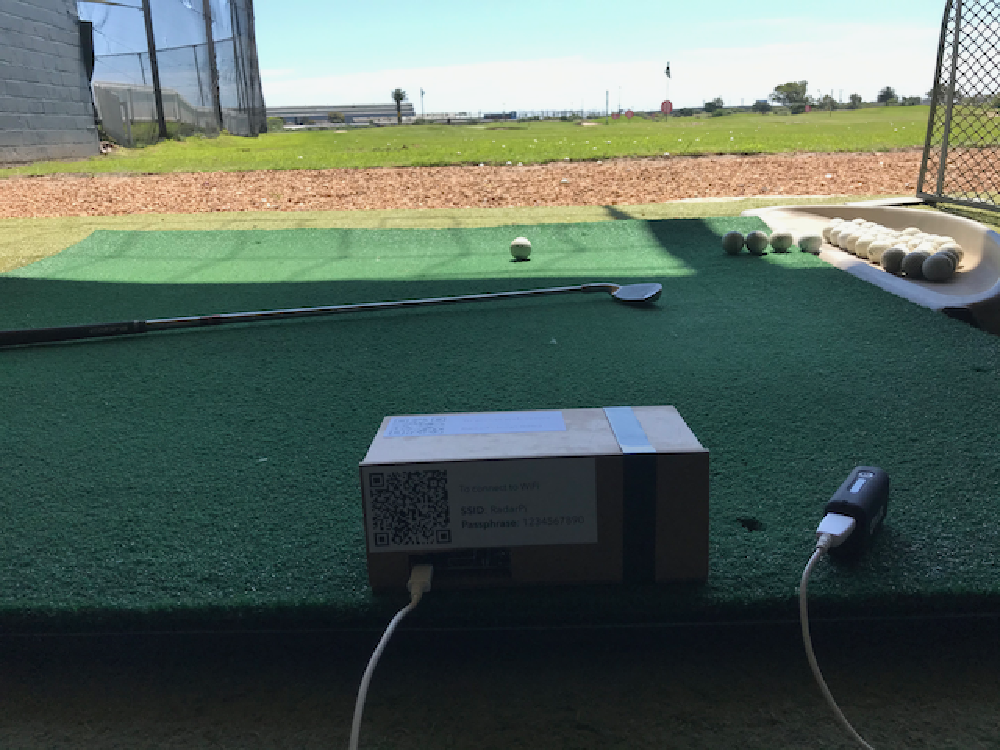
\includegraphics[width = 0.9\textwidth]{images/golfball.pdf}
    \caption{Setup of radar behind golf ball}\label{fig:golfball}
    \end{minipage}\hfill
    \begin{minipage}{0.45\textwidth}
        \centering
        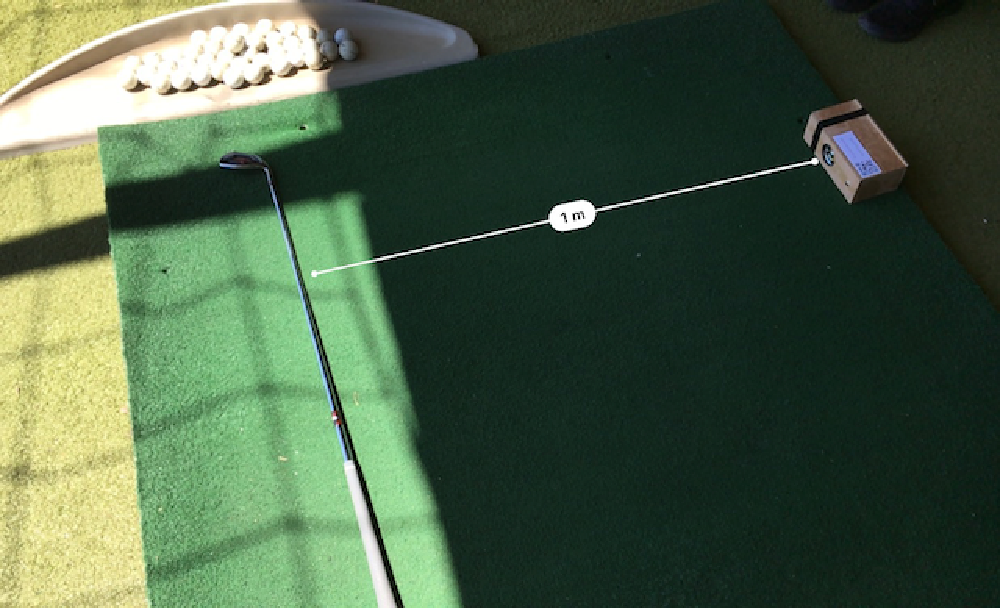
\includegraphics[width=0.9\textwidth]{images/measuregolf.pdf}
        \caption{Radar $1\ m$ behind the golf ball}\label{fig:measuregolf}
    \end{minipage}
\end{figure}

\subsubsection{Result}
Figures \ref{fig:cw2results} and \ref{fig:cw2results2} shows the results from the test described above. The results show two different attempts. Figure \ref{fig:cw2results} shows the results obtained with $9000\ Hz$ and Figure \ref{fig:cw2results2} shows the results as obtained with $7000\ Hz$.

\begin{figure}[h!]
    \centering
    \begin{minipage}{0.45\textwidth}
        \centering
        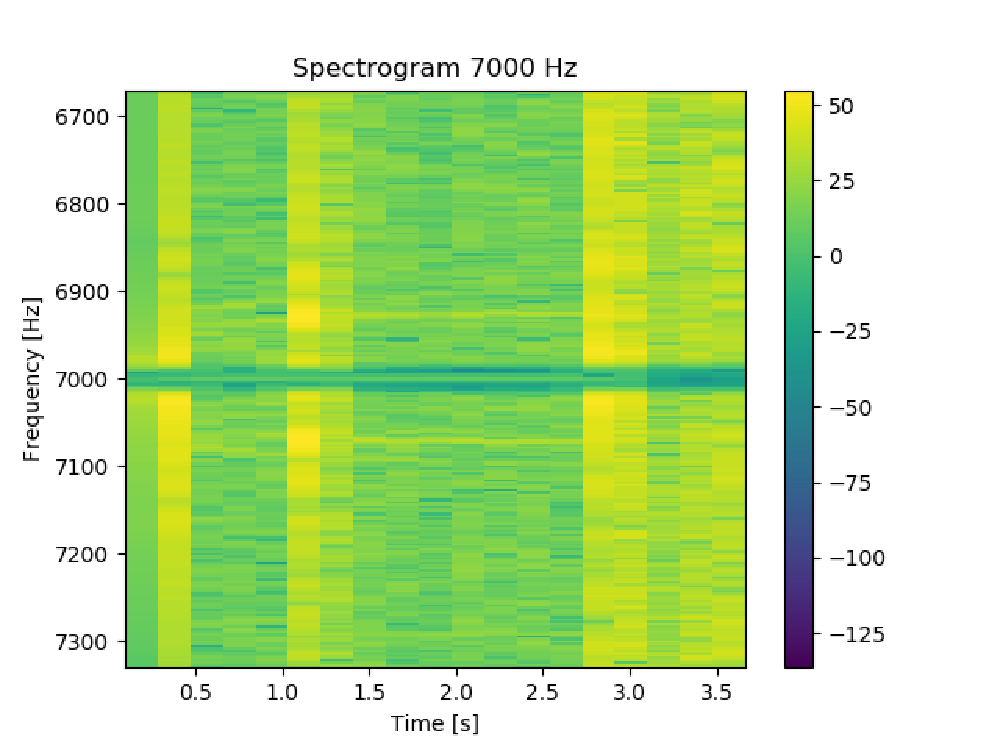
\includegraphics[width = 0.9\textwidth]{images/cw2results.pdf}
    \caption{CW Results of Golf club velocity 1}\label{fig:cw2results}
    \end{minipage}\hfill
    \begin{minipage}{0.45\textwidth}
        \centering
        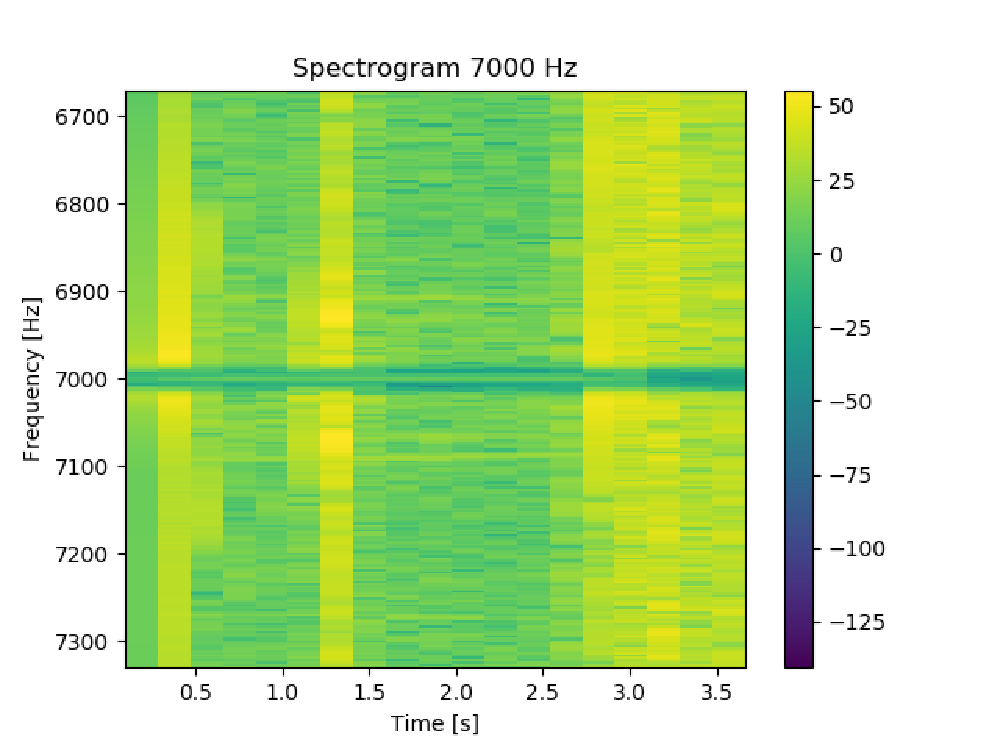
\includegraphics[width=0.9\textwidth]{images/cw2results2.pdf}
        \caption{CW Results of Golf club velocity 2}\label{fig:cw2results2}
    \end{minipage}
\end{figure}

\subsubsection{Discussion}
As shown in the results for this test, the resolution of the spectrogram proved to be difficult to read and make out exactly the velocity of the golf club. However, the backswing of the club is visible in the sixth bin and the forward hitting swing is also clearly visible toward the end of the spectrogram. The exact measurement of the club speed is not possible though. This can be due to the small size and small window that the golf club is within the beamwidth of the microphone. 

\section{Pulsed-Doppler}
\subsection{Test 1}
\subsubsection{Setup}
The radar was set up on top of a stool approximately $1.5\ m$ tall in the middle of a room on the top floor above a standard $2$ vehicle garage. The dimensions of the room are $6$ m x $7.2$ m  with a floor space of $43.2\ m^2$ and feature a staircase coming up from below. The floor plan can be seen in Figure \ref{fig:floorplan}.

\begin{figure}[h!]
    \centering
    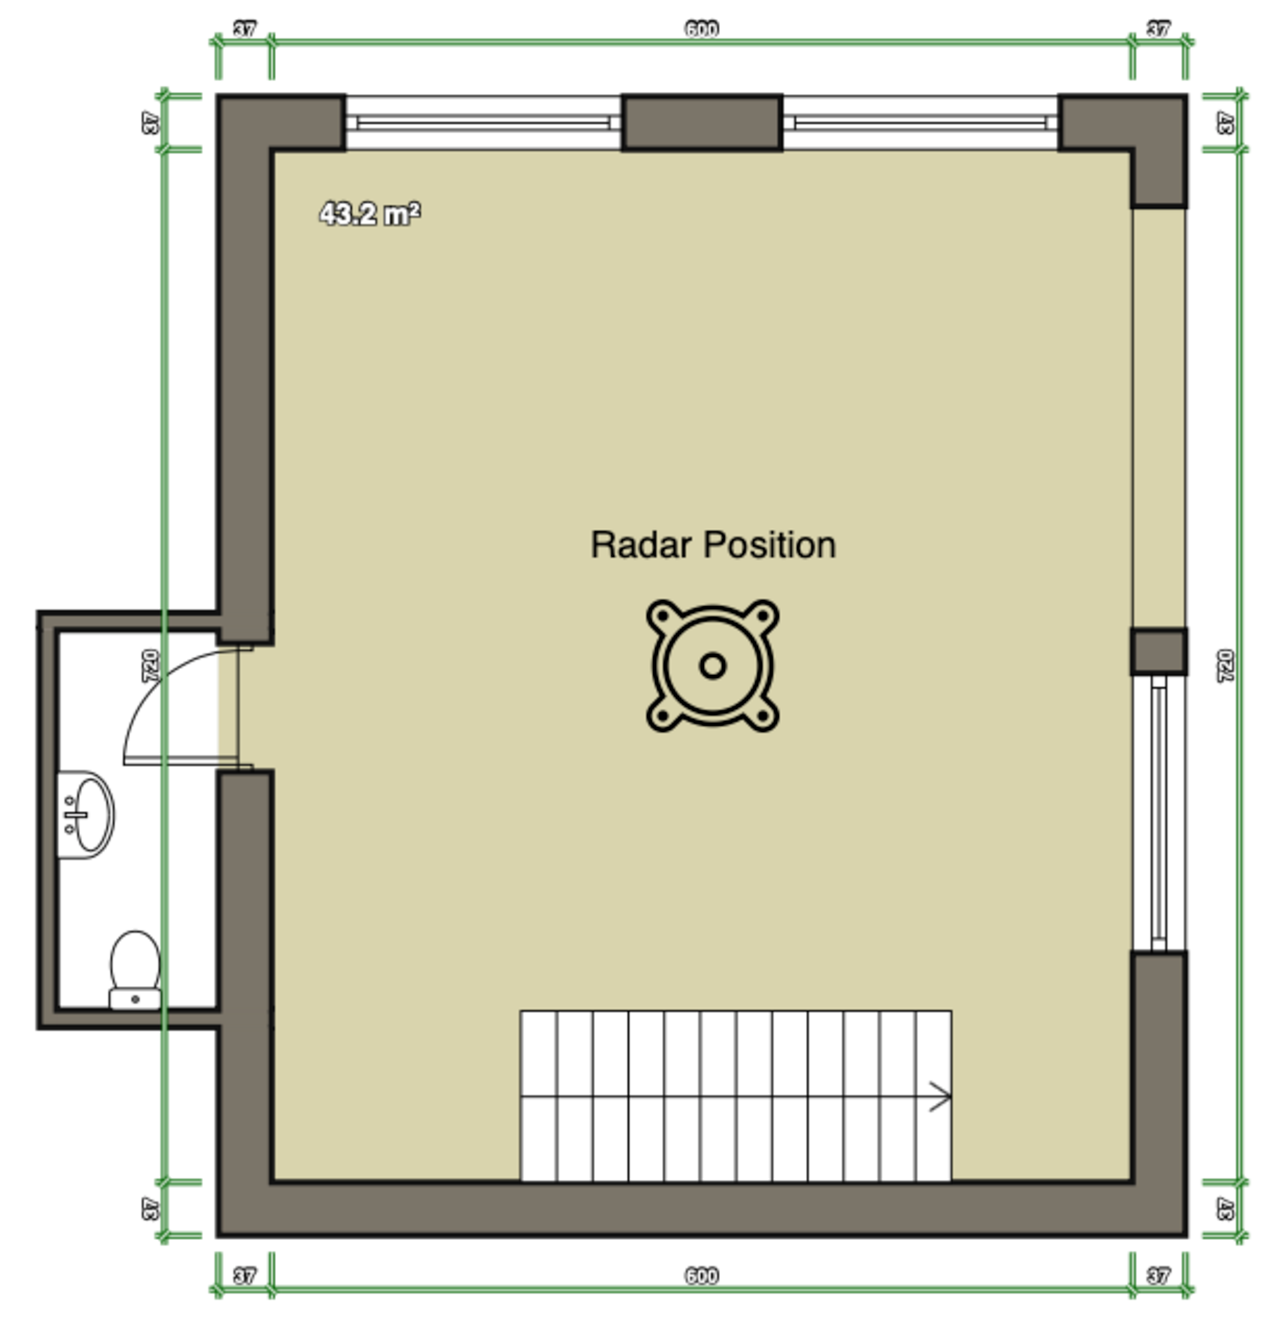
\includegraphics[width = 0.6\textwidth]{images/floorplan.pdf}
    \caption{Floorplan setup for PD Radar Test 1}\label{fig:floorplan}
\end{figure}

Figure \ref{fig:setupPDTest1} shows the physical location of the radar.

\begin{figure}[h!]
    \centering
    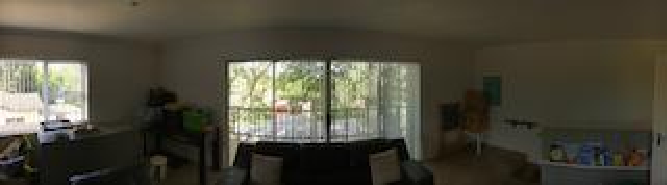
\includegraphics[width = 1\textwidth]{images/setupPDTest1.pdf}
    \caption{Radar setup for PD Radar Test 1}\label{fig:setupPDTest1}
\end{figure}

\subsubsection{Result}
The test was conducted four times, once to each flat part of a wall. This should be enough to map the dimensions of a simple rectangular room. The results in Figures \ref{fig:pulsedTest1-1} and \ref{fig:pulsedTest1-2} only shows the distance to the northern wall and the Western wall. The remaining results can be seen in Appendix \ref{appendix:PDResults}.

\begin{figure}[h!]
    \centering
    \begin{minipage}{0.45\textwidth}
        \centering
        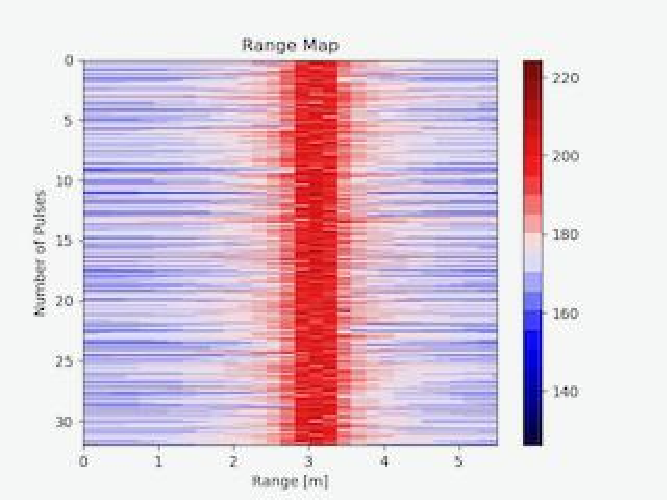
\includegraphics[width = 0.9\textwidth]{images/pulsedTest1-1.pdf}
        \caption{Measurement to the Northern Wall}\label{fig:pulsedTest1-1}
    \end{minipage}\hfill
    \begin{minipage}{0.45\textwidth}
        \centering
        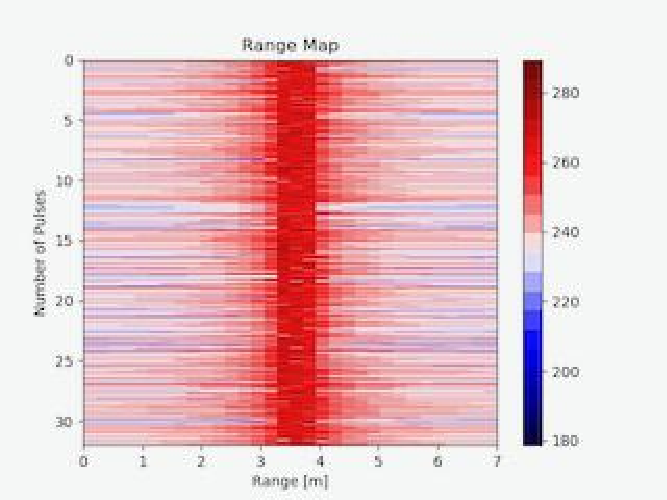
\includegraphics[width=0.9\textwidth]{images/pulsedTest1-2.pdf}
        \caption{Measurement to the Western Wall}\label{fig:pulsedTest1-2}
    \end{minipage}
\end{figure}

\subsubsection{Discussion}

The wall was measured to be approximately $3\ m$ from the radar to the Northern wall and approximately $3.5\ m$ to the Western wall. This corresponds to the floor plan and the measurements proved to be somewhat accurate although the range map shows quite thick amplification and an exact measurement proved to be difficult.

\subsection{Test 2}
\subsubsection{Setup}
The radar was set up on a bridge to measure the distance to the water. Figure \ref{fig:setupPDTest2} shows the bridge and Figure \ref{fig:pulsedTest22} the location of the radar on the bridge. The radar was handheld and operated using an iPad. The non-technical implementation of the radar was used with a maximum unambiguous range of $9\ m$ and a volume of $100\%$. 

\begin{figure}[h!]
    \centering
    \begin{minipage}{0.45\textwidth}
        \centering
        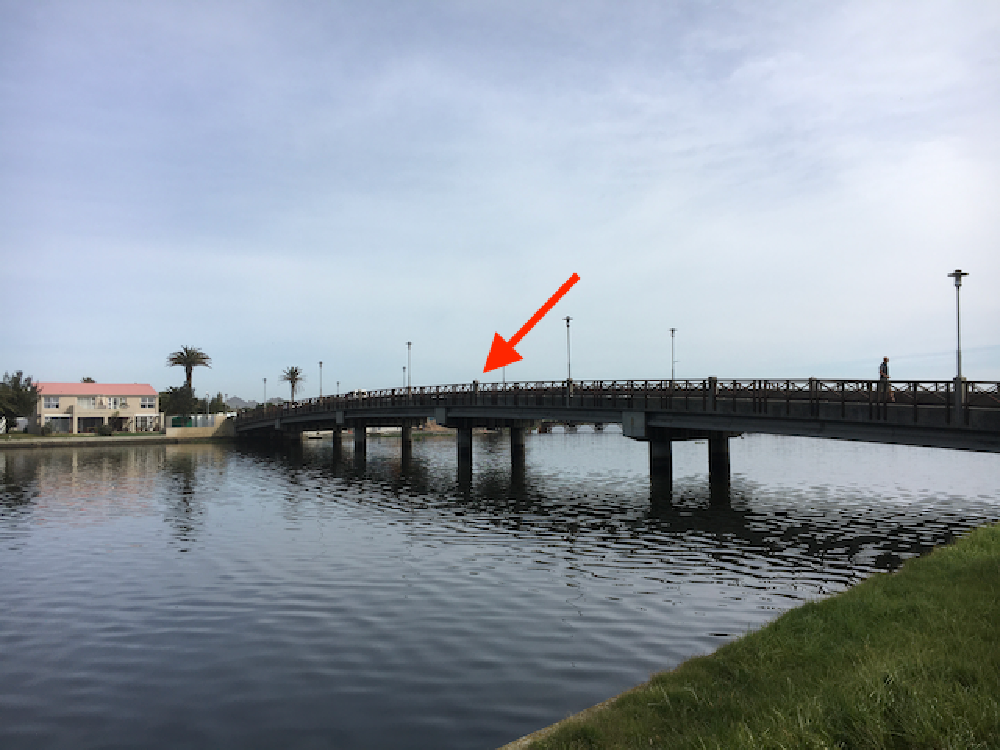
\includegraphics[width = 0.9\textwidth]{images/setupPDTest2.pdf}
    \caption{Setup of Radar on bridge}\label{fig:setupPDTest2}
    \end{minipage}\hfill
    \begin{minipage}{0.45\textwidth}
        \centering
        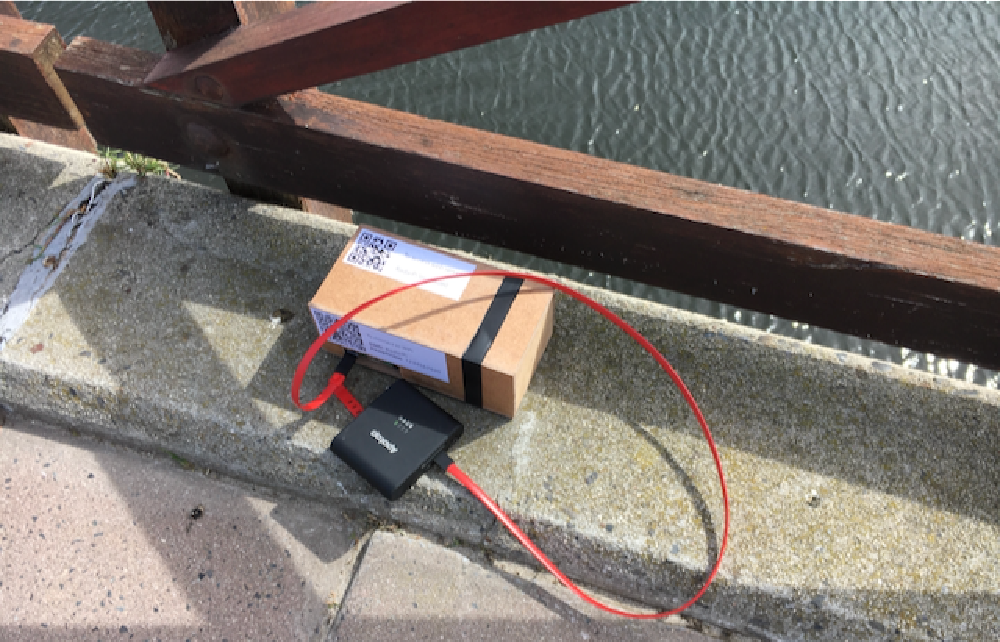
\includegraphics[width=0.9\textwidth]{images/setupPDTest22.pdf}
        \caption{Location of Radar on bridge}\label{fig:pulsedTest22}
    \end{minipage}
\end{figure}

\subsubsection{Result}
The results of the process laid out above, the measurement was taken and the results can be seen in Figure \ref{fig:setupPDTest2Results}.

\begin{figure}[h!]
    \centering
    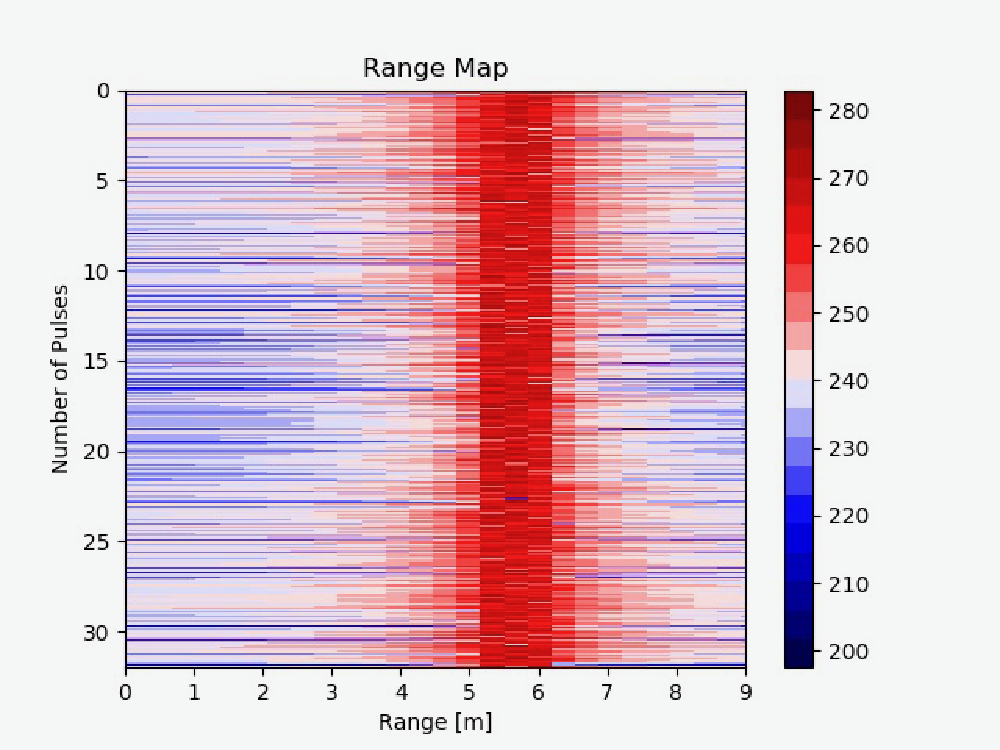
\includegraphics[width = 0.4\textwidth]{images/setupPDTest2Results.pdf}
    \caption{Distance to water measurement}\label{fig:setupPDTest2Results}
\end{figure}

\subsubsection{Discussion}

The results from above clearly show a range of $5\ -\ 6\ m$. Once again, the resolution is not great and accurate measurement can not be obtained. The bridge was quite noisy since it is used by cars and the nearby construction on the new bridge made taking measurements difficult.

\section{Consistency Tests}
Consistency tests were conducted to verify that running the tests under the same conditions and the same targets would yield the same results. 

\subsection{Continuous Wave Radar}
The setup was a box moving toward, back and forward again to the radar at high speed ($0.5\ s$ per movement over $1\ m$, i.e. $2\ m.s^{-1}$), the duration of $1.5\ s$ and a tone of the frequency of $10\ 000\ Hz$. The setup of the test can be seen in Figure \ref{fig:setupCWresults}.

\begin{figure}[h!]
    \centering
    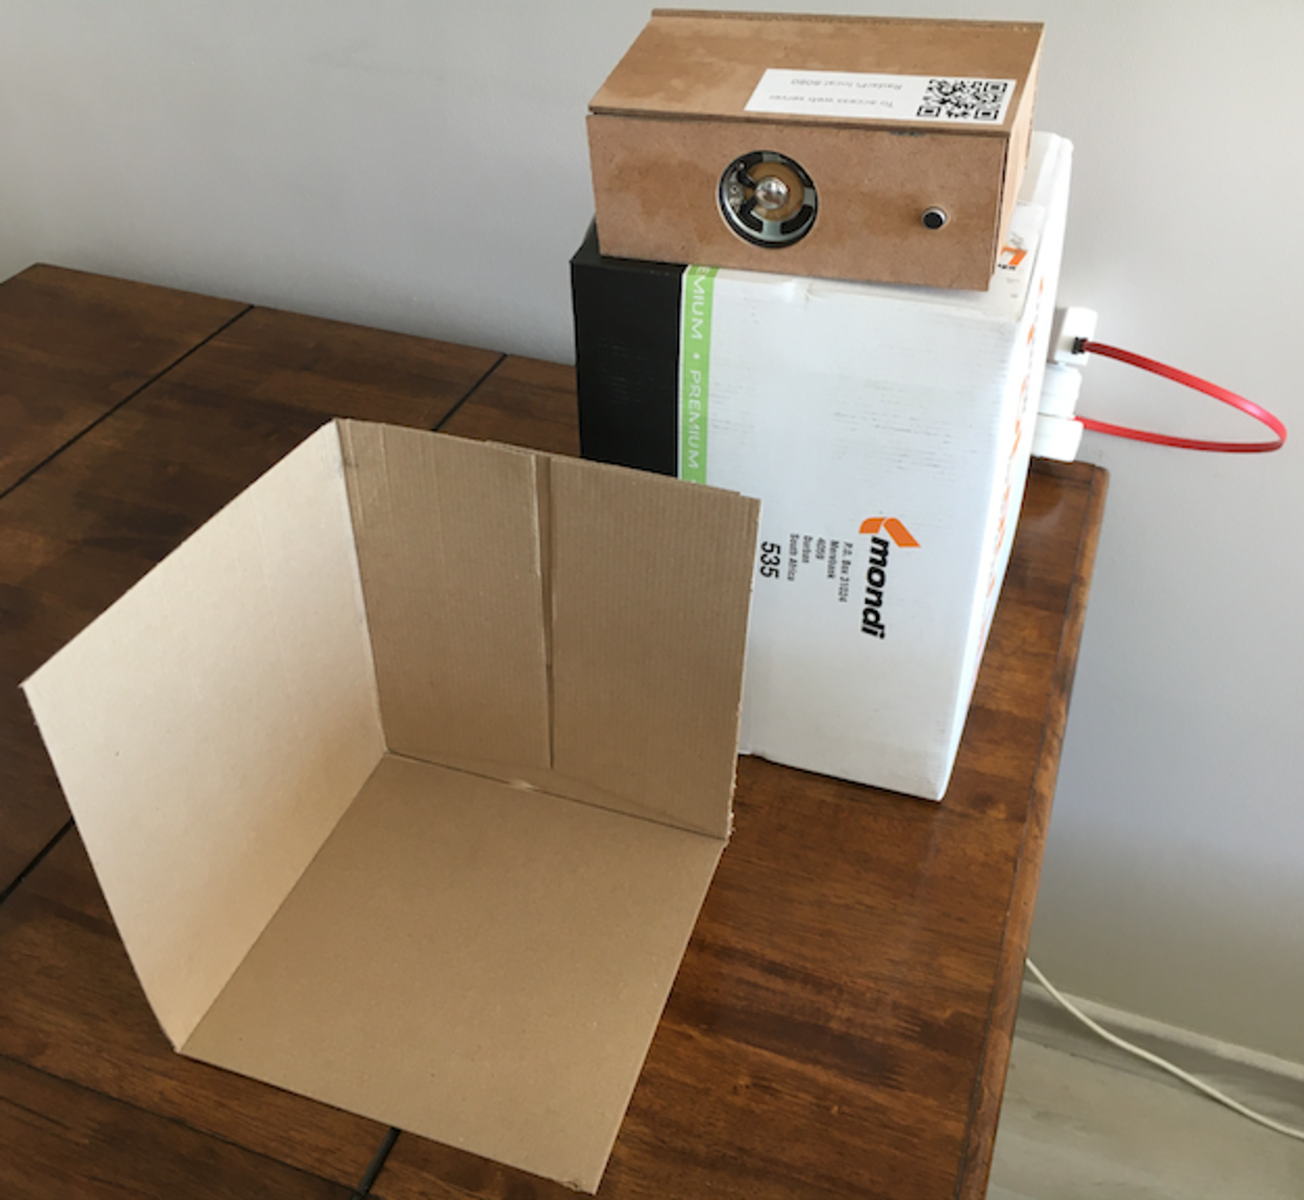
\includegraphics[width = 0.5\textwidth]{images/setupCWConsisresults.pdf}
    \caption{Setup of Radar on box and corner reflector for consistency tests}\label{fig:setupCWresults}
\end{figure}

Three tests were performed and the results are shown in Figures \ref{fig:CWResults1}, \ref{fig:CWResults2} and \ref{fig:CWResults3}.

\begin{figure}[h!]
    \centering
    \begin{minipage}{0.48\textwidth}
        \centering
        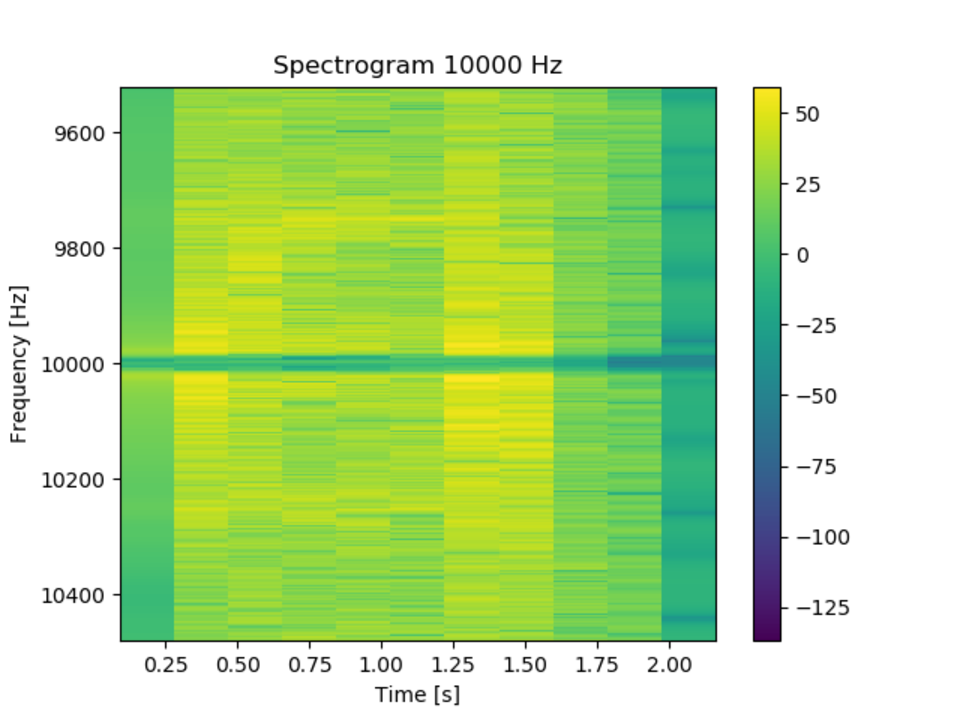
\includegraphics[width = 0.93\textwidth]{images/CWResults1.pdf}
        \caption{Front Facing View of Enclosure}\label{fig:CWResults1}
    \end{minipage}\hfill
    \begin{minipage}{0.48\textwidth}
        \centering
        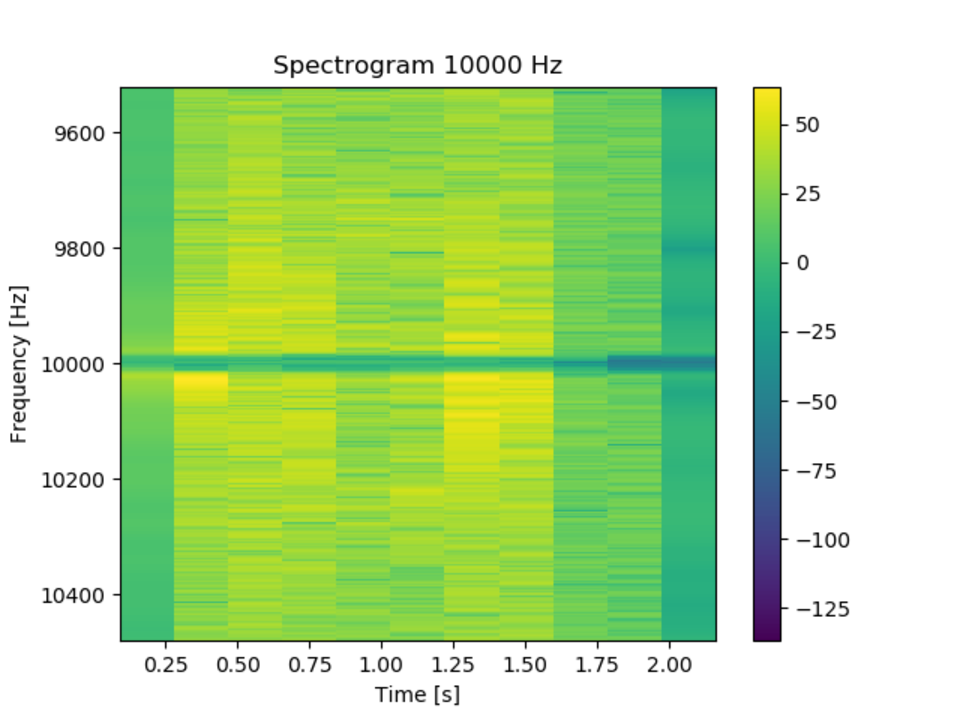
\includegraphics[width=0.93\textwidth]{images/CWResults2.pdf}
        \caption{Rear Facing View of Enclosure}\label{fig:CWResults2}
    \end{minipage}
\end{figure}

\begin{figure}[h!]
    \centering
    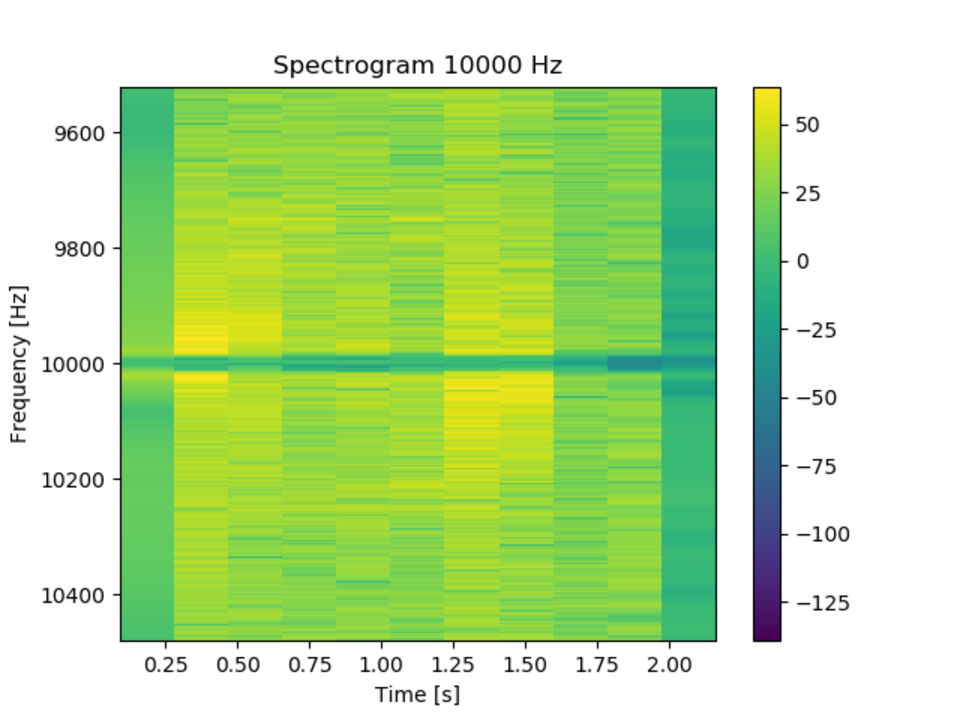
\includegraphics[width = 0.4464\textwidth]{images/CWResults3.pdf}
    \caption{Rear Facing View of Enclosure (Open)}\label{fig:CWResults3}
\end{figure}

\newpage
\subsection{Pulsed-Doppler Radar \label{section:PDResults}}
The setup was the radar hand-held at $1\ m$ away from a wall inside a parking lot with high ceiling and no nearby walls to minimise unwanted noise reflections. The parking garage was also selected so that minimal wind noise would impact the results. The setup of the test can be seen in Figures \ref{fig:setupPDresults} and \ref{fig:setupPDresults1}.

\begin{figure}[h!]
    \centering
    \begin{minipage}{0.45\textwidth}
        \centering
        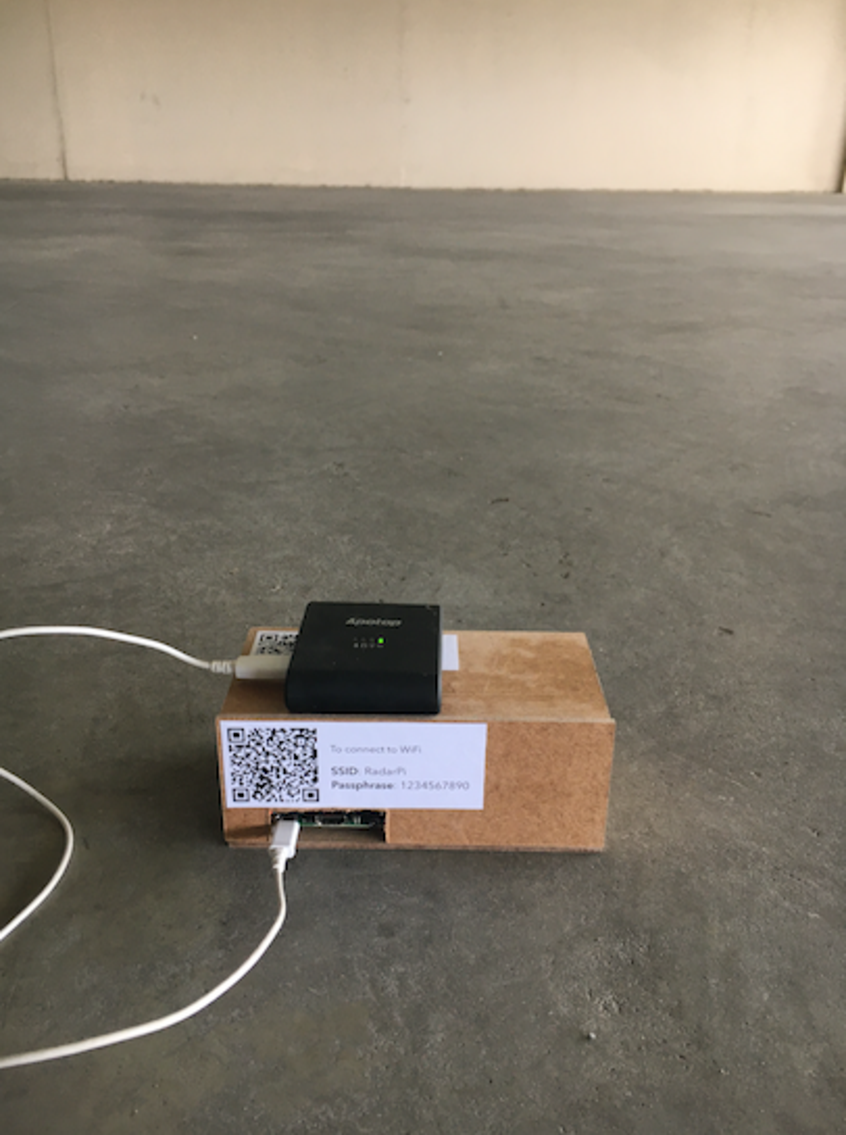
\includegraphics[width = 0.9\textwidth]{images/setupPDresults.pdf}
    \caption{View of the Radar to the wall}\label{fig:setupPDresults}
    \end{minipage}\hfill
    \begin{minipage}{0.45\textwidth}
        \centering
        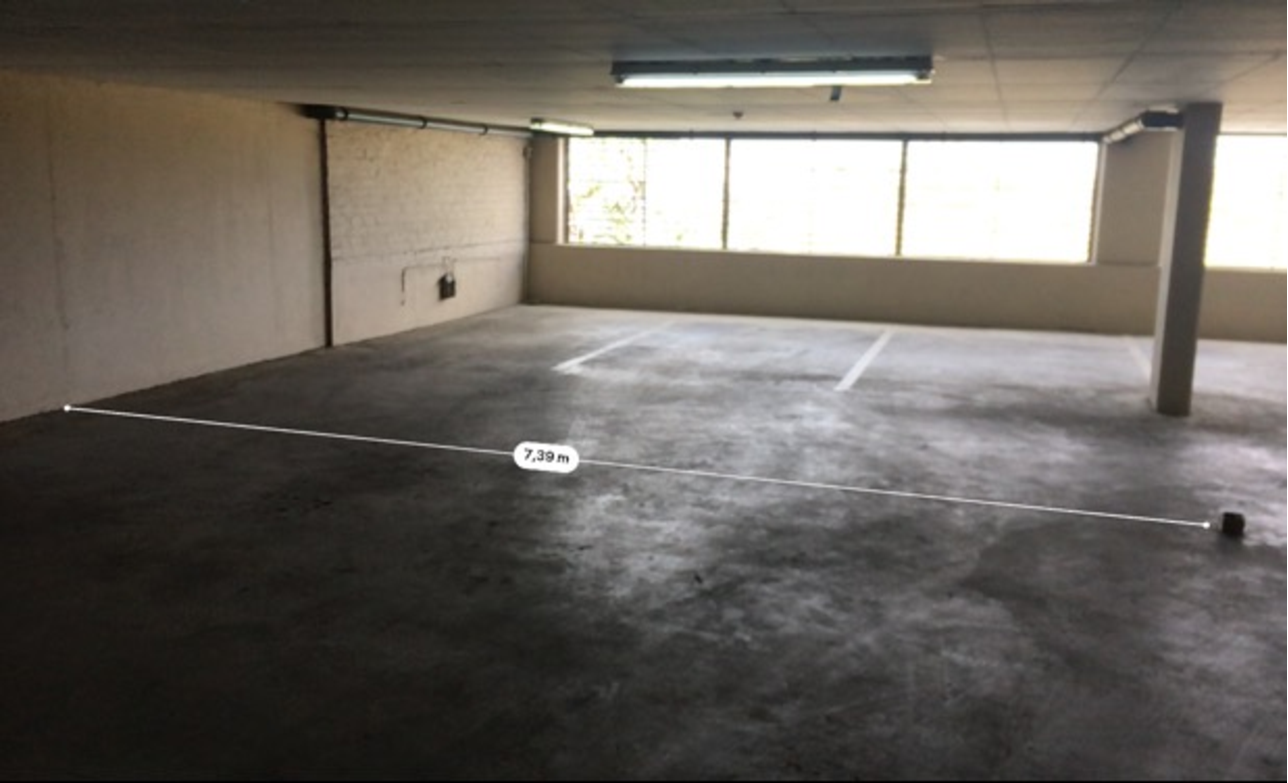
\includegraphics[width = 0.9\textwidth]{images/setupPDresults1.pdf}
    \caption{Distance measurement to the wall ($7.39\ m$)}\label{fig:setupPDresults1}
    \end{minipage}
\end{figure}

Three tests were performed and the results are shown in Figures \ref{fig:consistPDResults1}, \ref{fig:consistPDResults2} and \ref{fig:consistPDResults3}.

\begin{figure}[h!]
    \centering
    \begin{minipage}{0.48\textwidth}
        \centering
        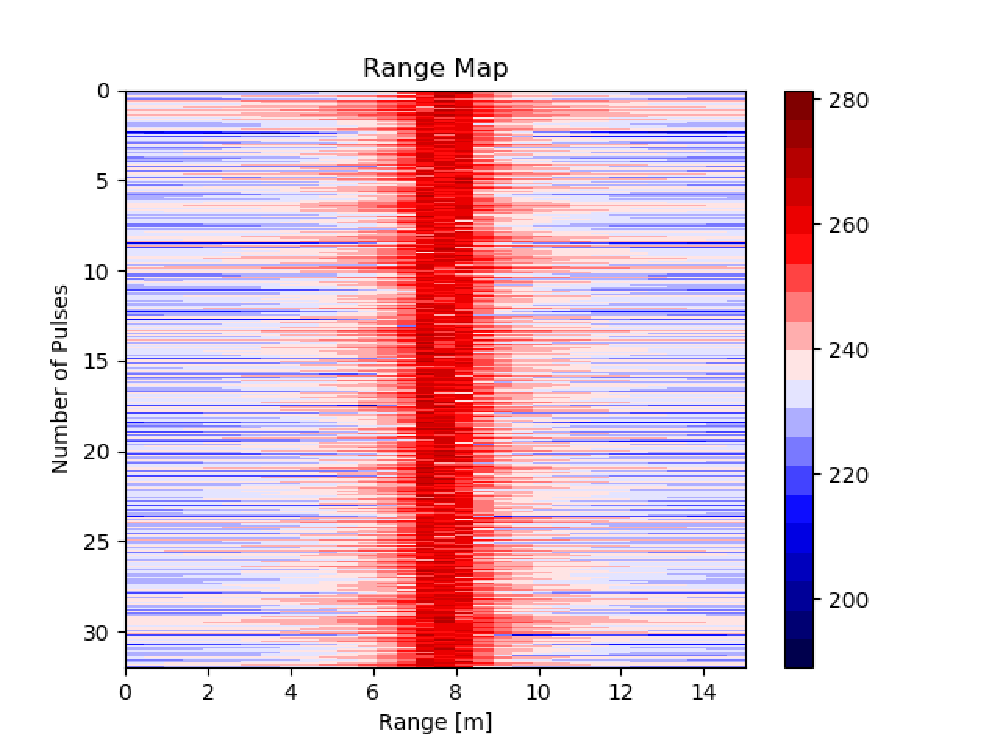
\includegraphics[width = 0.93\textwidth]{images/consistPDResults1.pdf}
        \caption{Pulsed-Doppler Consistency Test 1}\label{fig:consistPDResults1}
    \end{minipage}\hfill
    \begin{minipage}{0.48\textwidth}
        \centering
        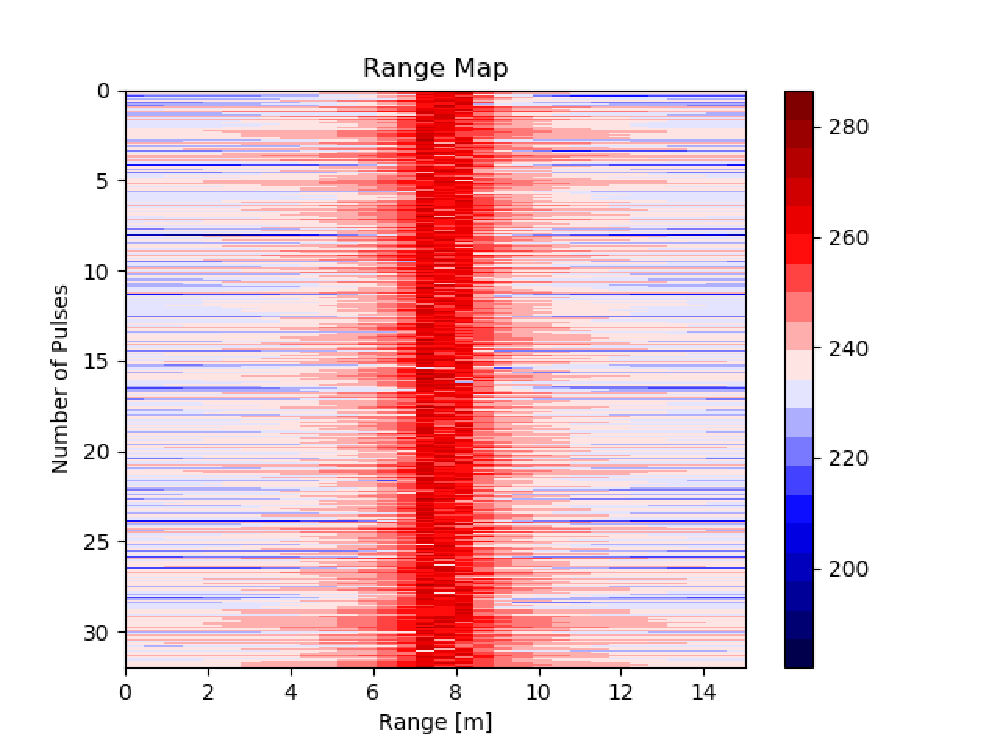
\includegraphics[width=0.93\textwidth]{images/consistPDResults2.pdf}
        \caption{Pulsed-Doppler Consistency Test 2}\label{fig:consistPDResults2}
    \end{minipage}
\end{figure}

\begin{figure}[h!]
    \centering
    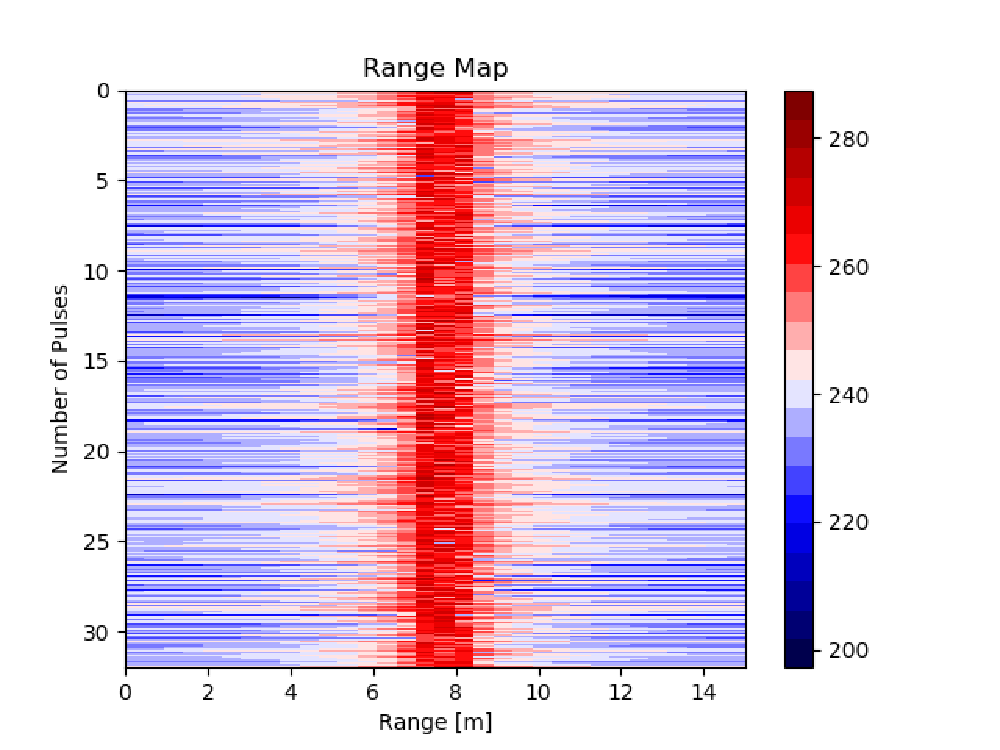
\includegraphics[width = 0.4464\textwidth]{images/consistPDResults3.pdf}
    \caption{Pulsed-Doppler Consistency Test 3}\label{fig:consistPDResults3}
\end{figure}



\subsection{Discussion}
As can be seen from the consistency checks performed above, the results are similar for both the continuous wave radar and the Pulsed-Doppler radar. 

The continuous wave radar is difficult to see exactly the velocity of the box moving toward and backwards from the radar but it differs significantly from a test where no movement has happened such as in Figure \ref{fig:notchApplied}. The results show similar movements and disturbances to the spectrogram. Therefore, the radar performed consistently over the three tests.

The Pulsed-Doppler radar tests all yielded similar results where the wall is recognised with similar returned power for all three tests. The leakage power that registers on the Range Map can be attributed to the parking garage reflections of sound although most precautions were taken to minimise the unwanted effects.

\newpage